\documentclass{article}
% preamble (Packages importieren)

\newcommand{\comment}[1]{}


\author{Eduard Scherer}
\title{Development \& Construction of an Autonomous Path-Following Drone}
\date{\today}
\usepackage[utf8]{inputenc}

\usepackage[
backend=biber,
style=numeric,
sorting=ynt
]{biblatex}
\addbibresource{references.bib} %Imports bibliography file

\usepackage{graphicx}
%\graphicspath{{C:\Users\eduar\Documents\Maturarbeit\MA-project\pictures}}
\usepackage{parskip}

\usepackage{listings}
\lstdefinestyle{BaselineStyle}
{ %
	commentstyle=\color{Blue},
	keywordstyle=\color{Green},
	numberstyle=\tiny\color{Gray},
	stringstyle=\color{Fuchsia},
	basicstyle=\ttfamily,
	columns=flexible,
	breakatwhitespace=false,
	breaklines=true,
	captionpos=b,
	keepspaces=true,
	numbers=left,
	numbersep=5pt,
	showspaces=false,
	showstringspaces=false,
	showtabs=false,
	tabsize=2,
	xleftmargin=1.5em,
	frame=single,
	framexleftmargin=1.5em
} %
% set to 'BaselineStyle'
\lstset{style=BaselineStyle}



% Dokument
\begin{document}
\maketitle
\tableofcontents
\pagebreak
	\section{Introduction}
	% TODO introduction
	% do at the end of the writing process
	% maybe a quick explanation of the term "drone"
	% drones are being used in war more and more self-built ones(Blheli32 is dead, because of the use in wars.)
	% article about more and more autonomous drones in the Ukraine-Russia War

	\section{Personal Motivation}
	\comment{rather short}
	\section{Literature Review}
	\subsection{General Software Considerations}
	% TODO work around the same topic that already exists
	
	There are three main softwares to consider when it comes to drones Betaflight, INAV and Ardupilot. All of them are open source. Multiwii is the origin of Betaflight and INAV. Multwii was Arduino based and then upgraded to Baseflight to be able to use the STM32 chips. Then it was forked to Cleanflight, which was later forked again into Betaflight and INAV\cite{history}. 
	
	The following three paragraphs are mostly based on \cite{firmwarearticle} and \cite{firmwarevideo}.
	
	Betaflight is in general the go-to option for first person view drones, commonly known as FPV drones, for either filming or racing. It is the most beginner friendly out of the three, because it has a large community, which results in a wide range of tutorials. When a new board comes out it is normally made to be used with Betaflight. However Betaflight lacks the option for different types of vehicles and generally the automated features are less developed compared to the other two. 
	
	INAV offers basic autonomous flight using waypoints and automated landing. It does not only support quadcopters, but also boats, rovers, planes and wings. It has a similar interface to Betaflight so switching from one to the other is easier than switching to Ardupilot.
	
	Ardupilot basically offers everything the other two have to offer and more for example Submarines and VTOLs. It is not commonly used with FPV, yet you can if you want to. It is more complicated to get into, but as a trade off you will be able to customize everything to your will. It is also the only option for a companion computer like the RaspberryPi. A few years ago it was really expensive to start, because it only supported the Pixhawk family of flight controllers which cost several hundred Franks a piece. However in recent years it has began to support more and cheaper flight controllers.
	
	\section{Methodology}
	%only what has been done
	\subsection{Drone Overview}
	If you want to fly a drone you have two options available either you buy one or you built one. The second option is for people who are interested in tinkering with their electronics until they work, not only the better option but also the cheaper one.
	
	The main parts needed for a drone are the flight controller(Fc), the electronic speed controller(ESC), the receiver, the battery and of course the frame, in addition you can also add a GPS, LEDs and more. The flight controller and electronic speed controller are referred to as Fc and ESC. The Fc runs the chosen software and controls every other part in one way or another. It is directly connected to the ESC, which controls the motors and is connected to the battery. The Fc also communicates with the receiver and GPS if there is one. In my case there will also a RaspberryPi which also connects to the Fc.
	% TODO add a graphic which illustrates the connection between the parts
	  
	\subsection{parts}
	
	\subsubsection[Fc]{Flight Controller}
	There are two different kind of flight controller the All-in-one(AIO) and just a Fc. The AIO is not only a Fc but also the ESC in one board. This has the advantage of only needing one board instead of two or five. However if only parts of the ESC or the Fc are damaged you need to replace the whole board which is more expensive than replacing only the Fc or ESC. 
	
	Betaflight and INAV both support a wide variety of Fcs compared to Ardupilot which is only supporting a very specific sample of boards\cite{FcSupport}. They have the option of open and closed hardware. Because the open hardware Fcs are quite expensive, so I decided to go with a closed one. The chip used in Fcs is usually a STM32. There are multiple generations of it the mainly used ones are F4, F7 and H7. The F7 and H7 are much faster than the F4 chips so the decision was not that difficult to make. I then decided to go with the Kakute H7 v1.3 (MPU6000)\cite{KakuteH7} from Holybro, because it was ok in the price and available as a stack. It comes shipped with Betaflight so I will need to flash Ardupilot. 

	\subsubsection[ESC]{Electronic Speed Controler}
	There are two different kind of ESCs, 4in1 and single ESCs. If you use single ESCs you will need one for each motor instead of a single board for all of them. The advantage of 4in1 ESCs is that you do not need a power distribution board, because it is already incorporated in the ESC, and that it can come in a stack. A stack is a Fc and ESC mounted on top of each other. It normally comes with stack screws. The disadvantage is that if a part of the ESC is damaged you need to replace the whole board. What needs to be looked upon buying a ESC is that the peak current of the motor is not higher than the burst current of the ESC, because it could damage a two high current could damage the ESC.
	
	My decision was to go with a 4in1 on a stack, because it is slightly cheaper and normally easier to wire. The only option with the Kakute H7 was the stack with the Tekko32 4in1 with a continuous current of either 50, 60 or 65 Ampere. I chose the 50A\cite{Tekko32} one, because you do not need a high continuous current rating when flying rather slowly and the motors I chose have a peak current of around 42A. 
	
	At the time I bought the ESC it was still shipped with BLHeli32 which as mentioned has seized their operations. I could however flash AM32 onto it.

	\subsubsection{Motor}
	There are two types of motor brushed and brushless ones. The difference between the two types is that the brushed motors are mechanically driven and the brushless motors are electrically driven. Therefor brushless motors also need an ESC to function compared to brushed ones. Brushed motors are used in really small drones with 1S batteries. However even in the small drones brushless motors are the more popular choice\cite{brush/lessmotors}. 
\begin{figure}[h]
	\centering
	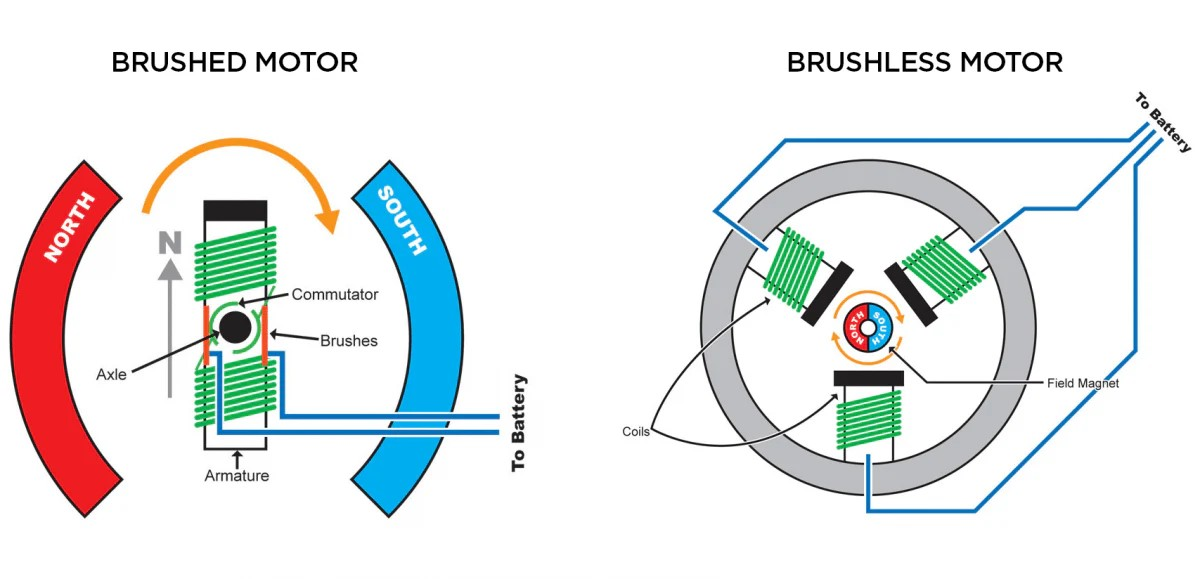
\includegraphics[scale=0.2]{pictures/motor}
	\caption{\cite{picturemotor}}
	\label{fig:motor}
\end{figure}

	The numbers that are seen on the motors like 2207 are describing the stator of the motor itself. In the case of a 2207 that would be 22mm diameter and a height of 7mm. The usual stator sizes of 5 inch drones are either 2207 or 2306. There is also the KV value which has to be considered. The KV value is the number of revolutions per minute(rpm) a motor turns when one volt is applied. The lower the KV value the more efficient is the motor and the higher the KV value the more responsive it is. The KV value for a 5 inch drone with a 4S battery is between 2300 and 2800. I chose the Iflight Xing-E Pro 2207\cite{xingepro} with a KV value of 2450, because the IFlight-Xing motors are known to be of good quality. 


	
	\subsubsection{Battery}
	There are two main types of batteries lithium polymer(LiPO) and Lithium-ion(Li-ion) batteries. LiPo batteries have a tendency to go up in flames. They have compared to the Li-ion batteries a much higher discharge rate, also seen as C value, so they are well suited for racing drones. However Li-ion batteries have a higher energy density, which means that they can store more mAh with the same weight as LiPo batteries, so they are more used in long range flying. The batteries have normally multiple cells, for example a 4S LiPo batterie contains 4 cells. This is important, because the more cells you have the higher is the voltage and so you will need a motor with a lower KV value. 
	
	I first wanted to buy two Li-ion battery packs, however they are hard to get and much more expensive. The other option would have been to solder them together myself, but it requires some soldering skill, which I did not have then. So I decided to go with 4S LiPo batteries from the Tattu R-line with 120C and 2000mAh\cite{tattu}, because I want something that can fly longer than just three or four minutes. I chose the brand Tattu, because it was the only known brand that was on AliExpress from where I got all the other components, so it seemed to be easier to also chose a battery from there. 
	
	\subsubsection{GNSS(Global Navigation Satellite System)/Compass}
	There are two different kinds of GNSS\footnote{The GNSS is usually referred to as GPS even though GPS is only the American GNSS system} modules the normal GPS/Compass boards and real time kinematic(RTK) GPS. Usually the chips used in both the RTK GPS and the normal GPS are from Ublox. The RTK GPS can achieve a accuracy of 1cm by incorporating information correction data from a RTCM, short for radio technical commision for maritime\footnote{It was first used for the positions of boats and other vessels}. However the correction data is either subscription based, is not guaranteed to cover all of the area or you need to build one yourself, which is quite complicated\cite{rtkgps}. For a small drone it is also not worth it to have a RTK GPS that costs several hundred Franks instead of a GPS with a 2m CEP which costs less than 30 Franks. Some of the GPS units also have a compass built-in so you will not need to buy an extra compass when using ArduPilot. 
	% TODO Explanation box for CEP
	
	I chose the Holybro Micro M10 GPS\cite{holybrom10micro}, because it comes from the same brand as the Fc and will be easier to connect. In addition to that the M10 chip is the newest version of Ublox chips and it would be senseless to buy an older version. It also is at least as good as other better-known GPS as the Matek M10Q\cite{gpstest}. It also comes with a built-in compass.	

	\subsubsection{Radio/Transmitter}
	The following information about transmitter protocols is based on two videos\cite{transprotocols}\cite{mlrs}.
	\subsubsection*{FrSky}
	There are three FrSky protocols that are not compatible with each other ACCST, ACCESS and FrSky R9 ACCESS. ACCST has a range of around 1-2 km in open air. The firmware is built into almost all radios. It has a good latency but not as good as the other options. ACCESS is the successor to ACCST and has about the same range, but a lower latency, however not a class leading one. FrSky R9 ACCCESS gives you a range of over 50km in ideal condition. Unfortunately, the FrSky ACCESS porotcols are only supported by FrSky radios. There is one problem with FrSky. It is quite a difficult to manage, because of the three protocols that are not compatible with each other.
	% TODO Latency box
	\subsubsection*{TBS Crossfire/Tracer and Immersion RC Ghost}
	TBS Crossfire has a range of over 100km and is easy to use. It is also well tested and stable and has a good latency. 
	TBS Tracer can have also over 10km, but drains the battery when flying further away. It is more focused on racing due to the low-latency.
	Immersion RC Ghost as a range of over 10km. It is possible to switch between a low-latency for racing and a high-latency for long range flying. 
	\subsubsection*{ExpressLRS}
	ExpressLRS is the best in long range and in the combination of long range and latency. It has been shown by Wezley Varty\cite{elrswezley}\footnote{Due to him being fined by the Australian government he took down his own video, so here is a copy of it.} that it really can fly up to 100km\footnote{There are two version a 900MHz and a 2.4GHz and the main difference is that the 2.4GHz only at least over 30km but unlikely over 100km, but it has the lowest latency compared to any other protocol.}. It is together with mLRS the only two options who are open source.
	\subsubsection*{mLrs}
	The main difference between ExpressLRS and mLRS is that mLRS has a higher latency to send larger data packages to your telemetry device. Which is something that is needed if you want to adjust something or get more data from your drone over the Mavlink protocol during the flight. 
	
	\subsubsection*{Transmitter/Radio}
	I've decided to go with the Radiomaster RP4TD ExpressLRS 2.4GHz True Diversity Receiver\cite{radiomasterreceiver} on a recommendation of a friend. It also is compatible with mLRS if I want to switch later on.
	
	I went with the Radiomaster Boxer\cite{radiomasterboxer} radio, because it is somewhat in the middle range from radios and seems to be quite reliable and has many knobs to customize. 

	\subsubsection{Smoke Stopper}
	A part that stops the ESC from short circuiting due to wrongly soldered parts. It is there to prevent wrongly connected parts from burning and saves you quite a lot of money doing that. There are two groups of smoke stoppers one that you buy and gets destroyed when the ESC short circuits instead of the ESC. There is another category that does not destroy itself and there are also some that you can solder together on your own\cite{smokestopper}. 
	
	\subsubsection{Problems with the Parts}

	There were two problems that arose one less severe than the other. One problem was that my ordered Kakute-Tekko stack did not include stack screws, which they normally do. Stack screws are just screws that you can use to mount the stack onto the frame. So I needed to purchase them separately.
	
	The more severe problem I ran into was that the batteries from AliExpress were first held by the swiss border control and then I received two insect traps instead of batteries. Luckily I ordered one of the same batteries from Conrad, because the other two took too long to deliver.
	% TODO add pictures of the insect traps 
	
	\subsubsection{Propellers and Battery Charger}
	For the propellers(props) and battery chargers I went of the recommendations from AOS-RC and FPVknowitall. For the props I chose the Foxeer Donut 5145\cite{toroidal} and the HQ 5x4.3x3 V1S\cite{hqprops}. And for the battery charger I went with the cheapest option the 608 AC Lipo Battery Charger\cite{lipocharger}.

\subsubsection{Data Transfer Protocols}
	\subsubsection*{SPI}
	\subsubsection*{Uart}
	\subsubsection*{I2C}
	
	
	
	
	\subsection{soldering}
	
	\subsection{ardupilot}
	The following is based on the ArduPilot copter documentation\cite{ardupilotdocs}.
	\subsubsection{Ground Station}
	To configure ArduPilot there are multiple softwares so called ground stations(GCS) required. They are normally ground-based and can transmit data via with a wireless telemetry device or USB cable.  With the telemetry device they can also control the drone from the ground and alter the route it is autonomously flying. 
	
	The most widely used GCS is Mission Planner(MP)\cite{MissionPlanner} it is widely used, but runs only on Windows and Mac OS. It also has a wiki which helps you install it. I will use it for the first-time configuration of my drone. 
	
	Another GCS is MavProxy it is based on Python and is only for the Linux operation system(OS). Which is the OS I will have on my RaspberryPi companion computer. 
	
	There is also QGroundContrlol which is unique, because it supports next to Windows, Mac OS and Linux also Android and IOS.

	\subsubsection{Firmware Installation}
	
	For the first time installation I need to flash the Kakute H7 with ArduPilot, because it is shipped with Betaflight as mentioned earlier on. For that I downloaded the ArduPilot firmware\cite{ArduPilotFirmware} for the Kakute H7. Afterwards the STM32CubeProgrammer\cite{STM32CubeProgrammer}, to flash the firmware onto the Fc. I connected the Fc in DFU mode directly with the computer using a USB cable. Then selected the USB port with which the Fc is connected and flashed the Fc. A reboot to get out of the DFU mode was required before connecting the Fc to MP and saw the first Yaw measurements. The progress of flashing the firmware was straight forward which will not be the case for the rest of the configuration. 
	% TODO add an explanation box for the DFU mode.

\begin{figure}[h]
	\centering
	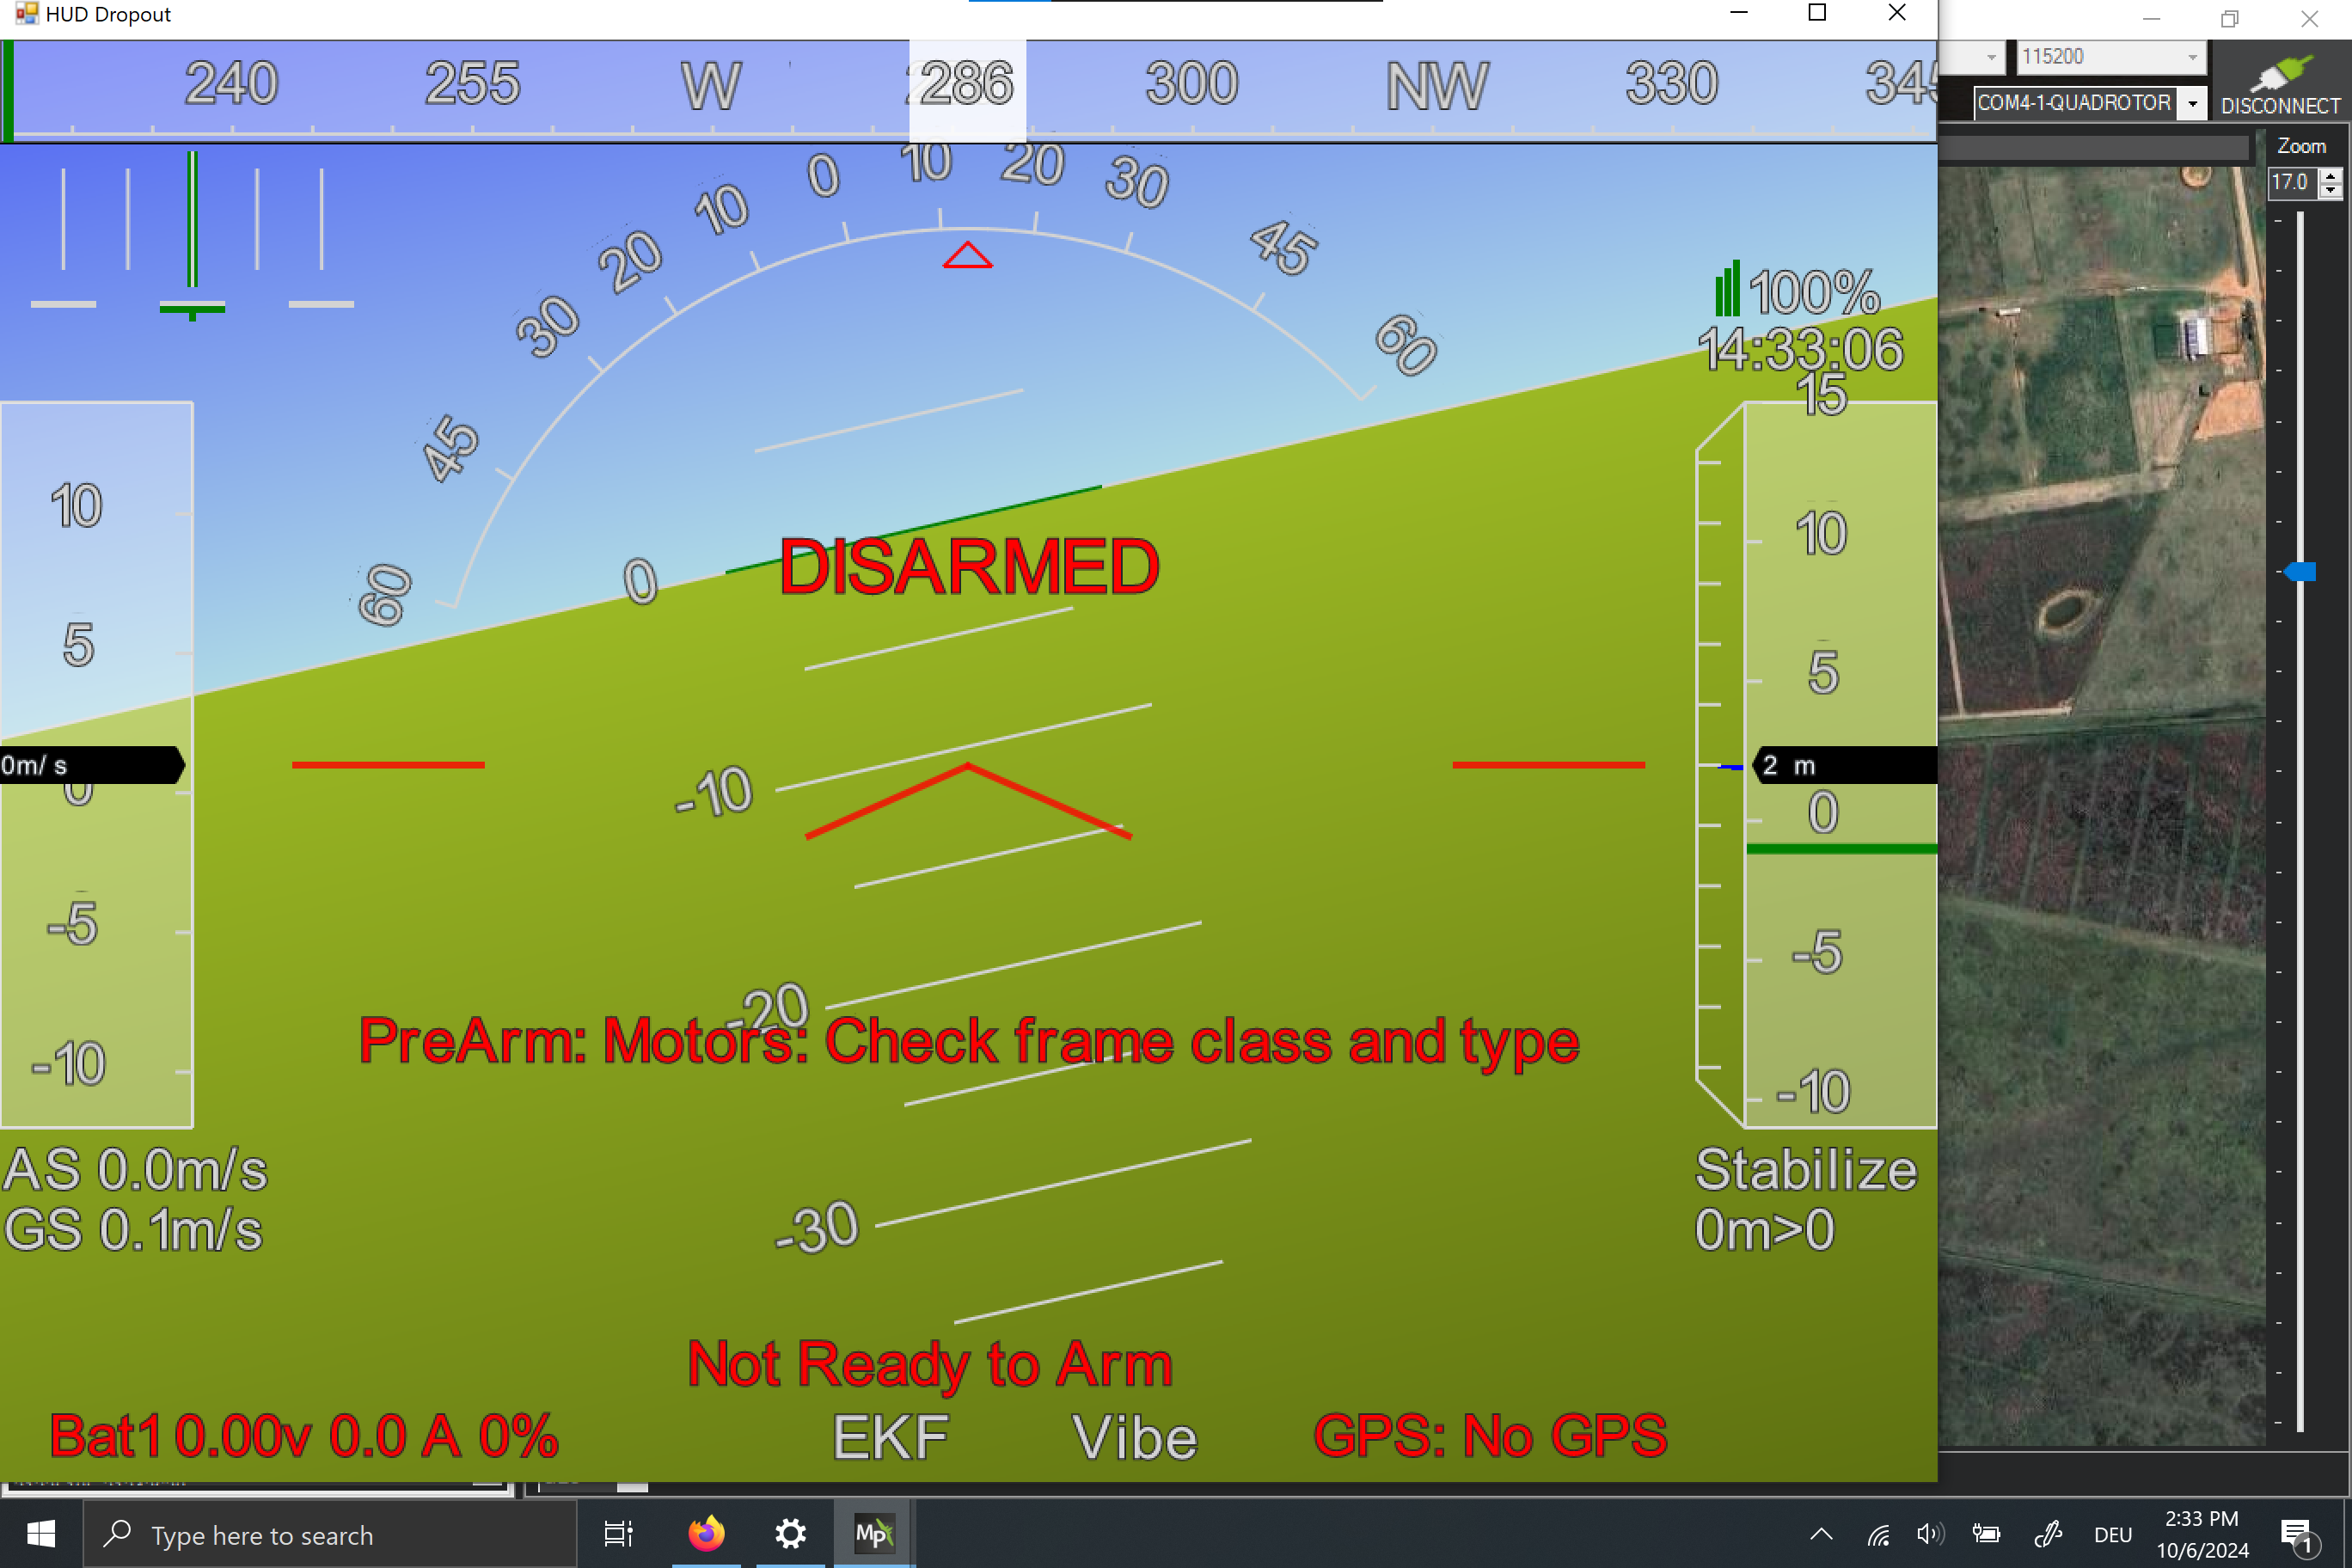
\includegraphics[width=0.7\linewidth]{pictures/Gyro_pos2_large}
	\caption{}
	\label{fig:gyropos2large}
\end{figure}
\begin{figure}[h]
	\centering
	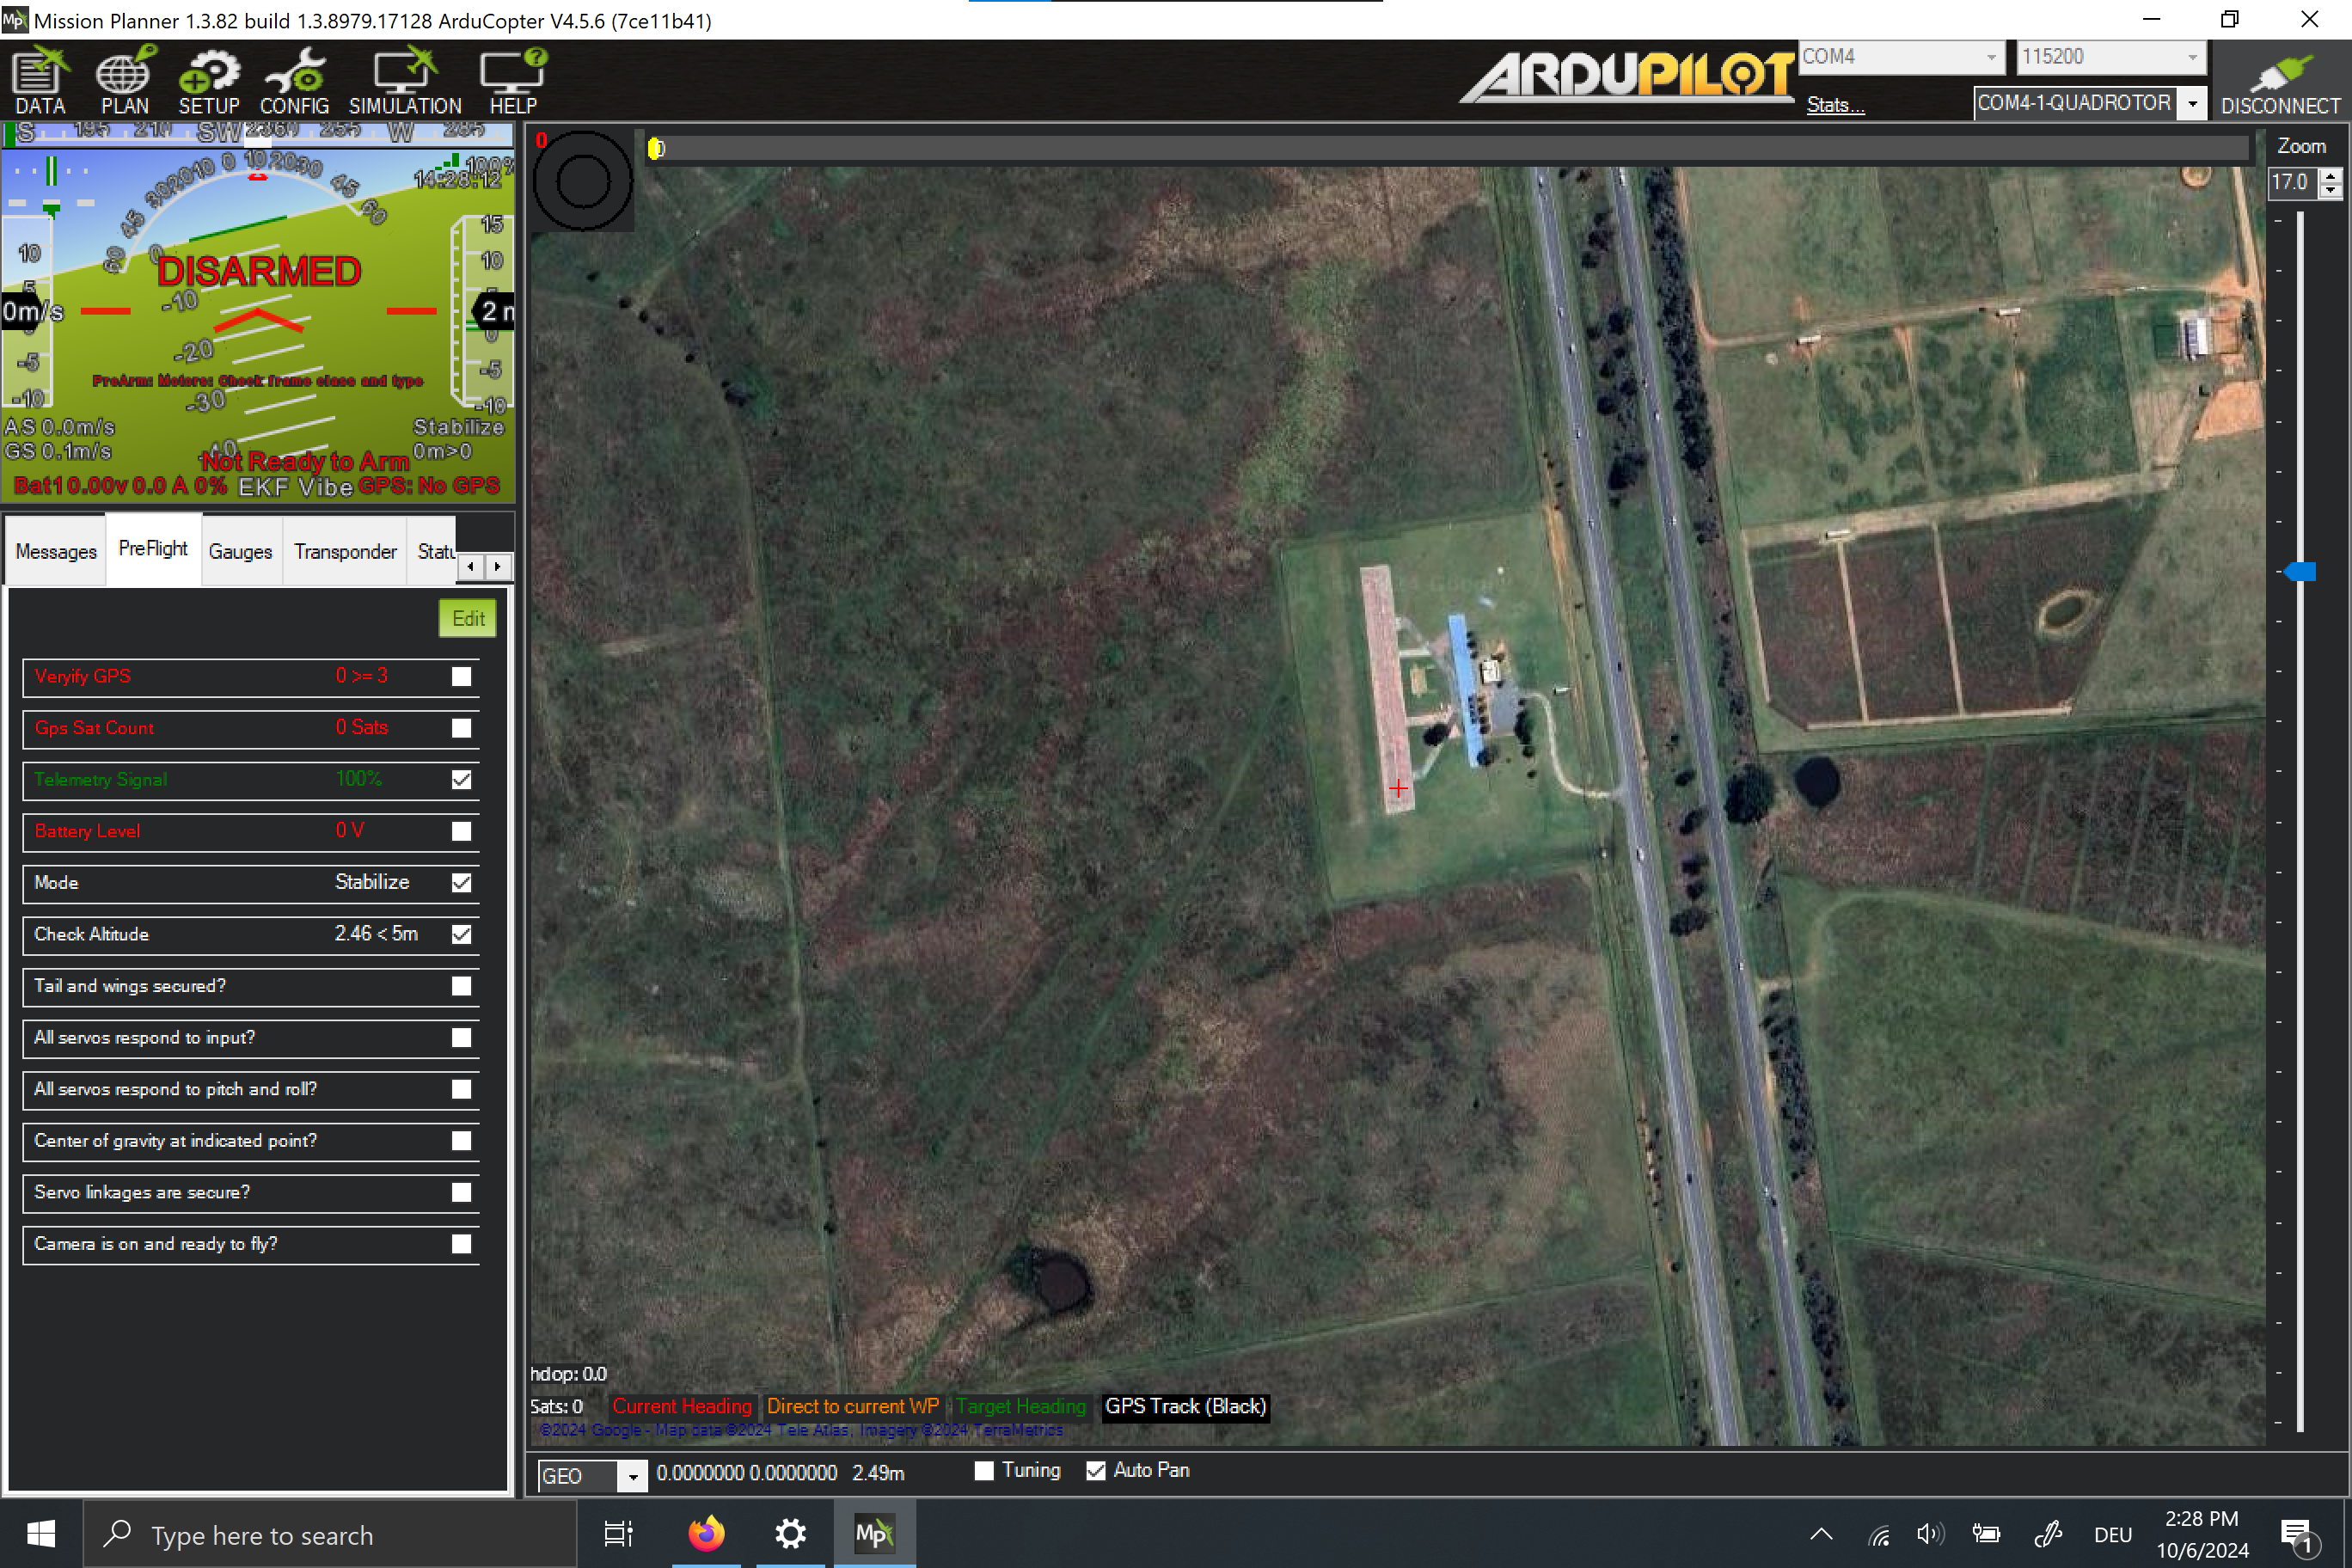
\includegraphics[width=0.7\linewidth]{pictures/Gyro_pos2.JPG}
	\caption{}
	\label{fig:gyropos2}
\end{figure}


	\subsubsection{GPS Connection}
	When I tried to get a GPS connection a No GPS message appeared. Changing the \lstinline|GPS_Type = 2| for the Ublox GPS did not change the No GPS error message.
\begin{figure}[h]
	\centering
	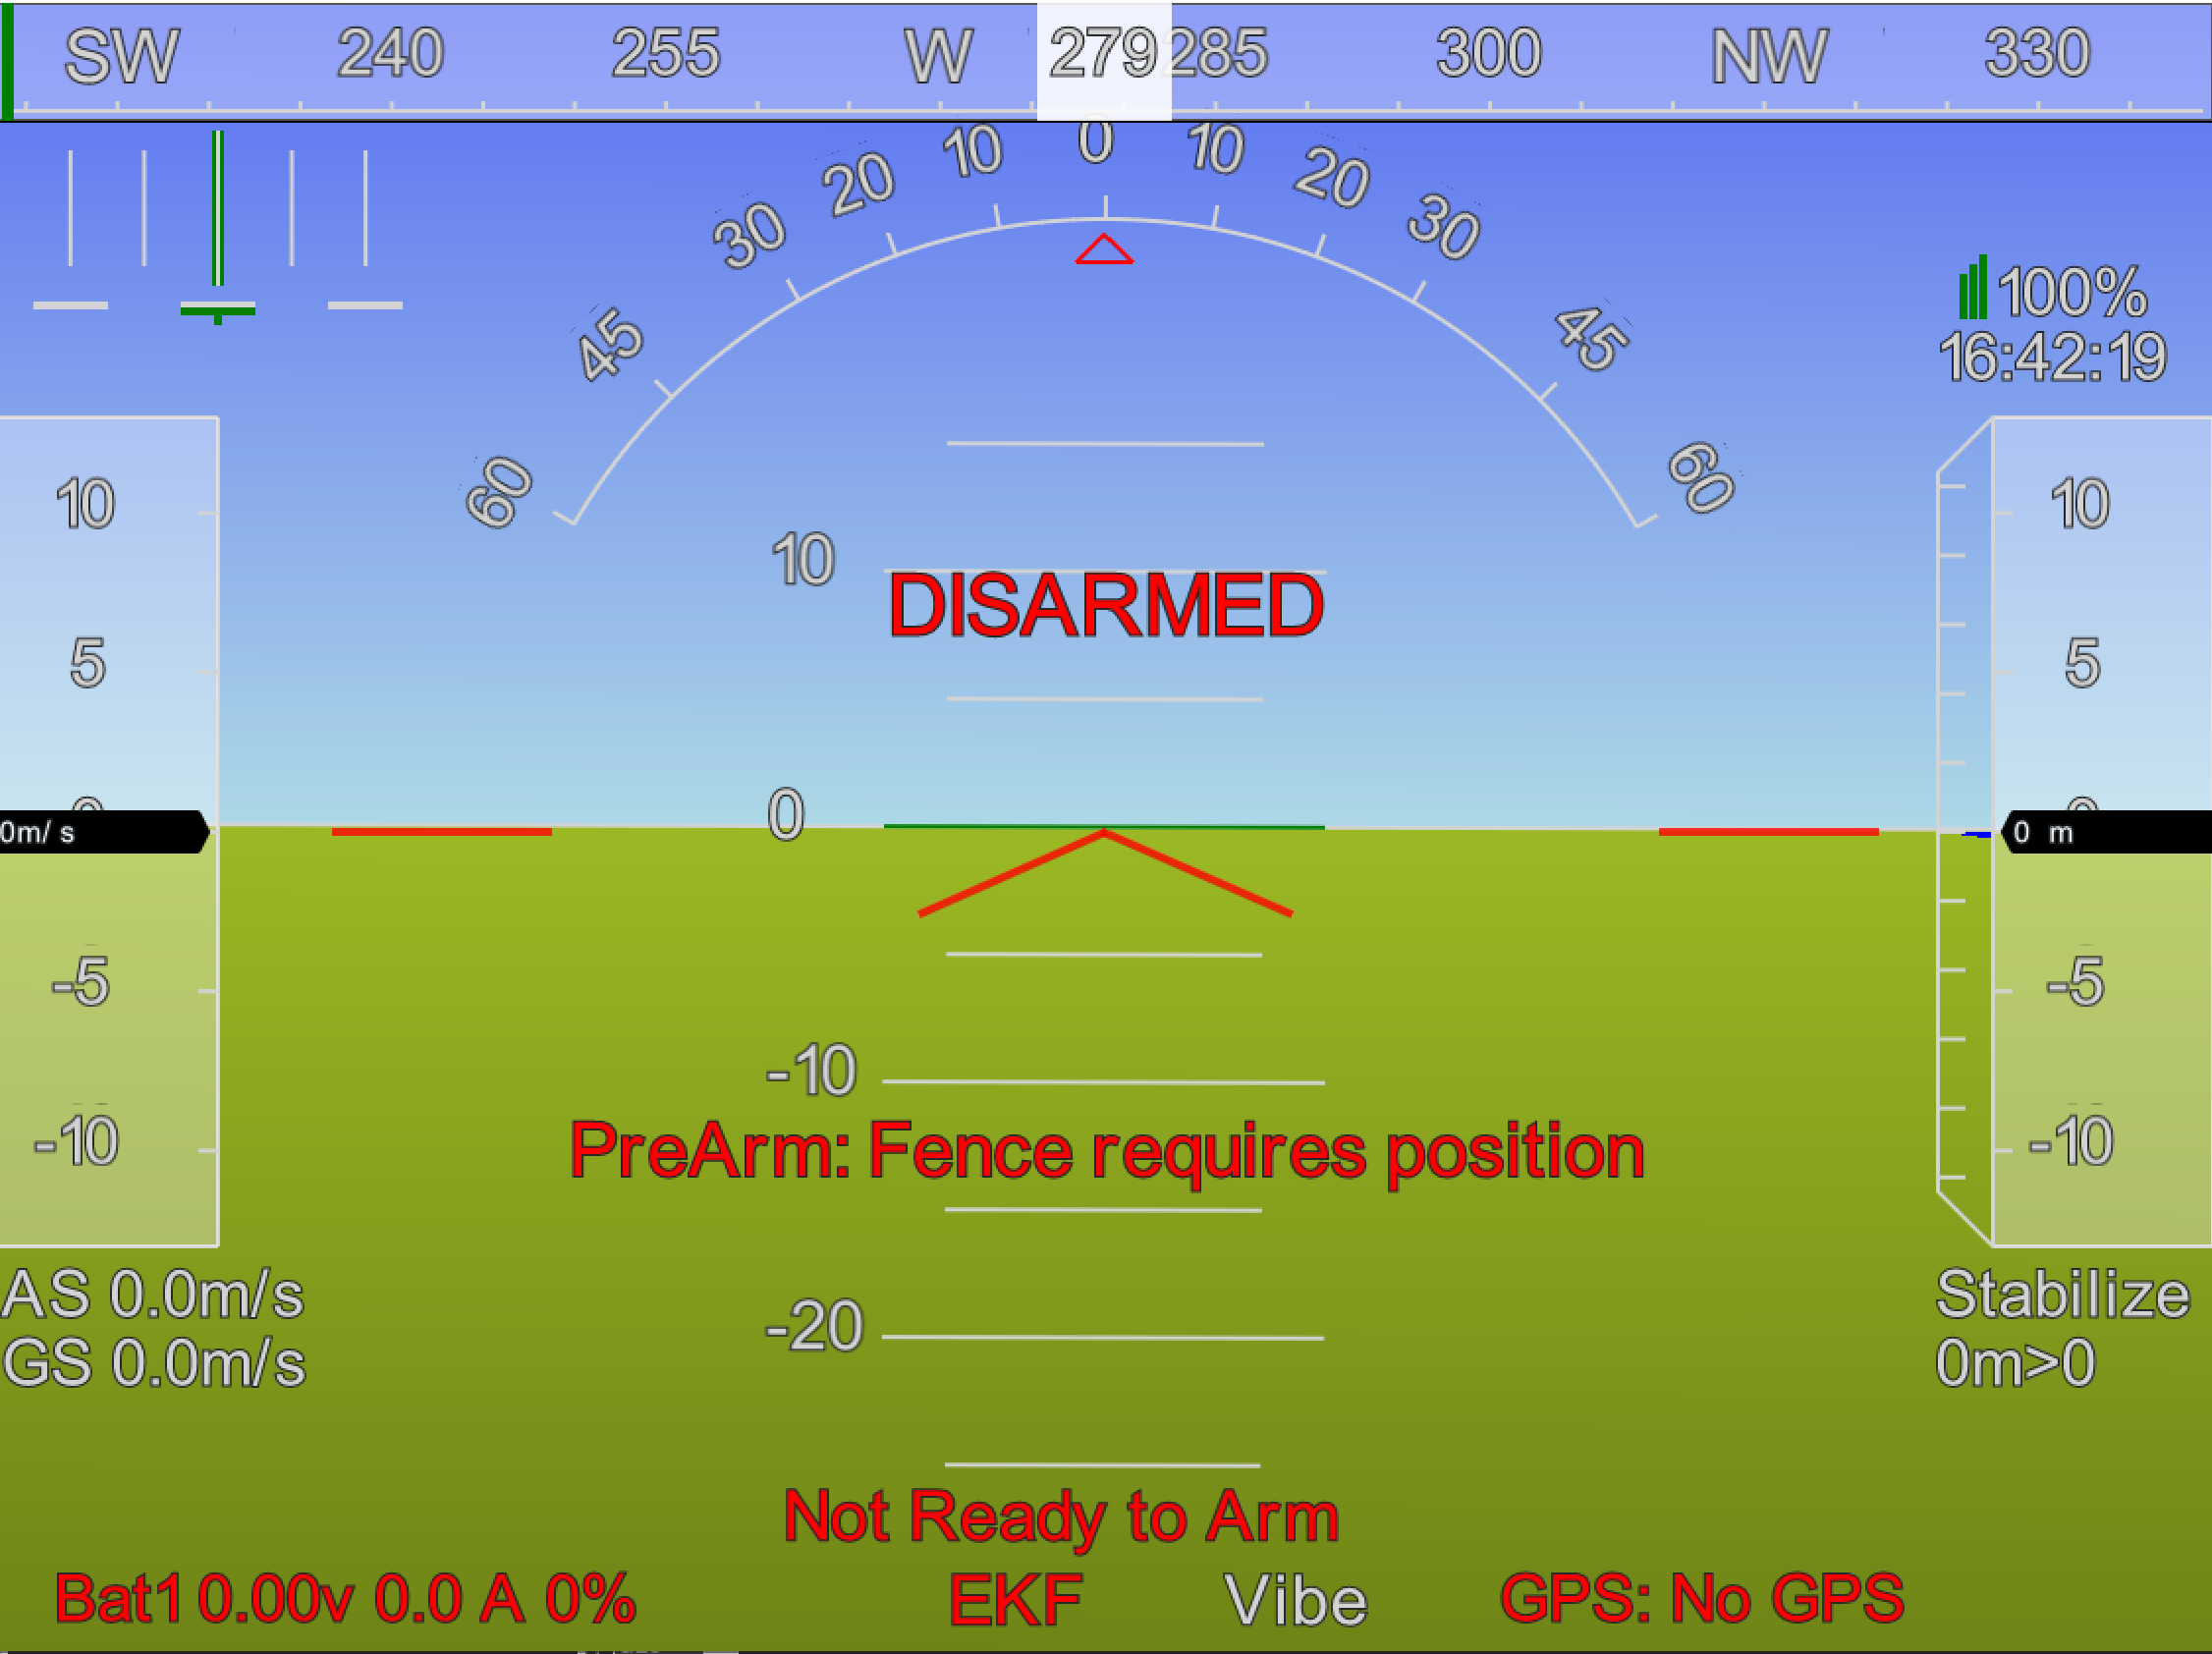
\includegraphics[scale=0.2]{pictures/No_GPS}
	\caption{}
	\label{fig:nogps}
\end{figure}

	Even though I was certain that the GPS worked well, because the compass of the GPS was already detected in the compass calibration tab.
	% TODO get better picture
\begin{figure}[h]
	\centering
	
\includegraphics[width=0.7\linewidth]{pictures/M10_compass_detected}
	\caption{}
	\label{fig:m10compassdetected}
\end{figure}

	I then went outside, away from metal tables and as far away from my computer that was possible with the USB cable it still did not show up in MP. I also checked the soldering and if the cables from the GPS to the Fc are connected correctly and both seemed fine. The GPS itself was not damaged, because the blue led was blinking constantly which means it is connecting to a GNSS.

	The problem was that the \lstinline|Serial3_Protocol|(Which is for the Uart3, which will be used for the connection to the RaspberryPi) was set to 5 which means GPS, however by being on 5 it blocked the Uart4, to which my GPS was really connected. After disabling the Uart3 it finally worked.

\pagebreak % temporary to have a better overview
	The GPS is quite precise outside. (Figure 6)
	%TODO add point on the picture where I'm really at
	
\begin{figure}[h]
	\centering
	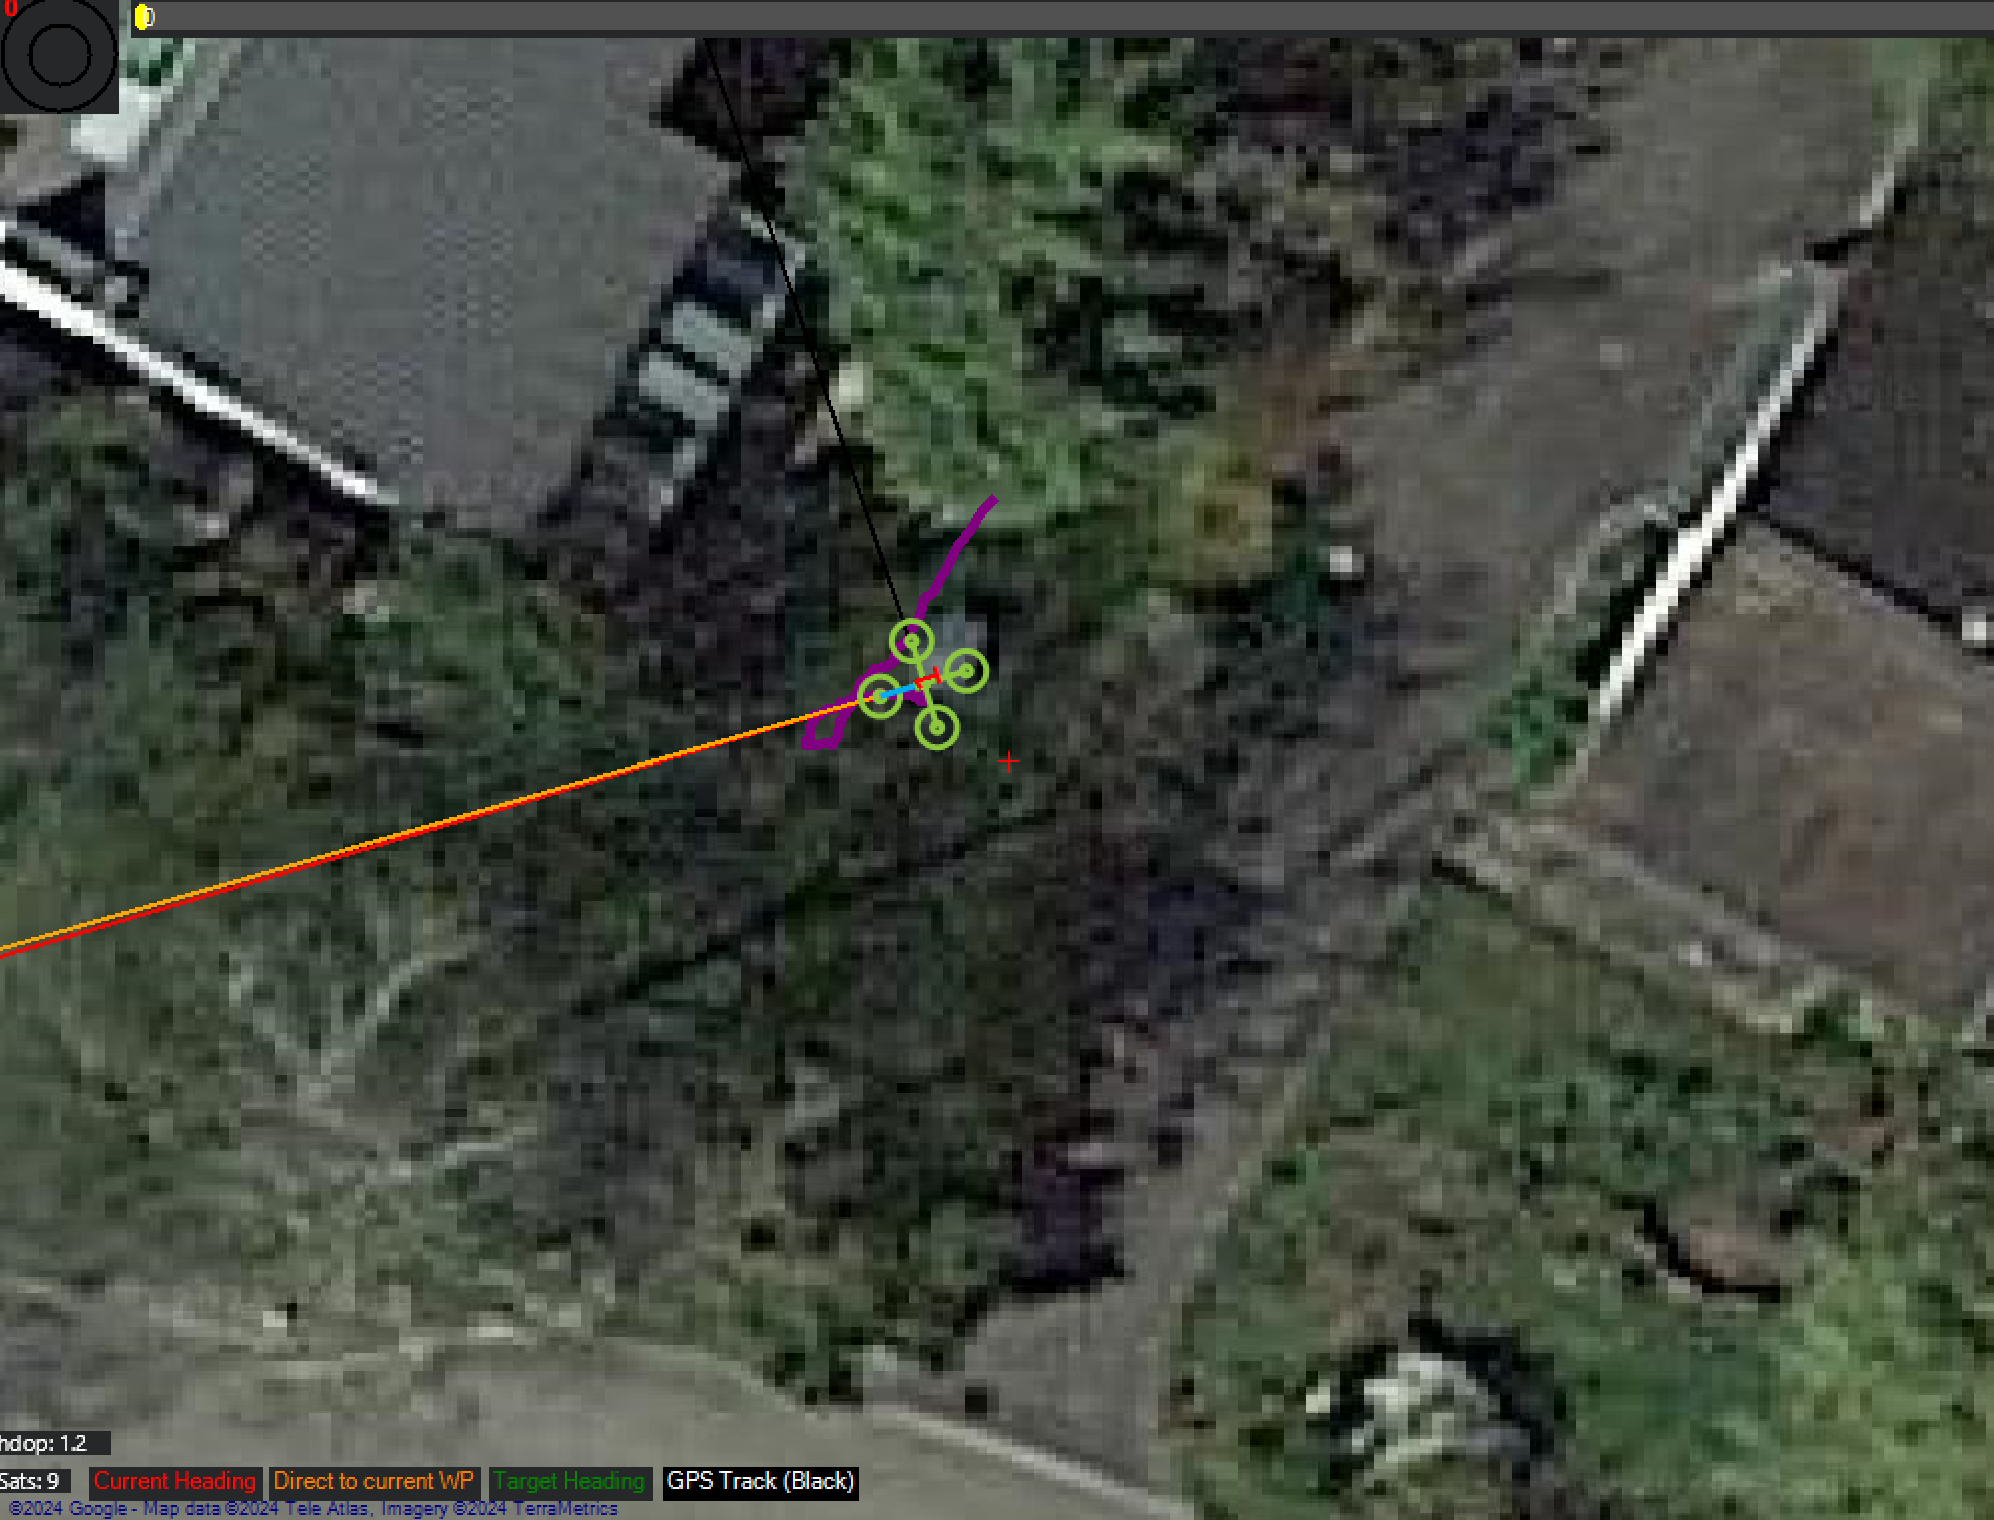
\includegraphics[scale=0.2]{pictures/GPS_Outside}
	\caption{}
	\label{fig:gpsoutside}
\end{figure}
	
	It also works sometimes inside and is precisely on my room, but sometimes it shows that I'm in Poland the middle of the Atlantic Ocean or Iceland.

	
\begin{figure}[h]
	\centering
	\begin{minipage}[b]{0.4\textwidth}
		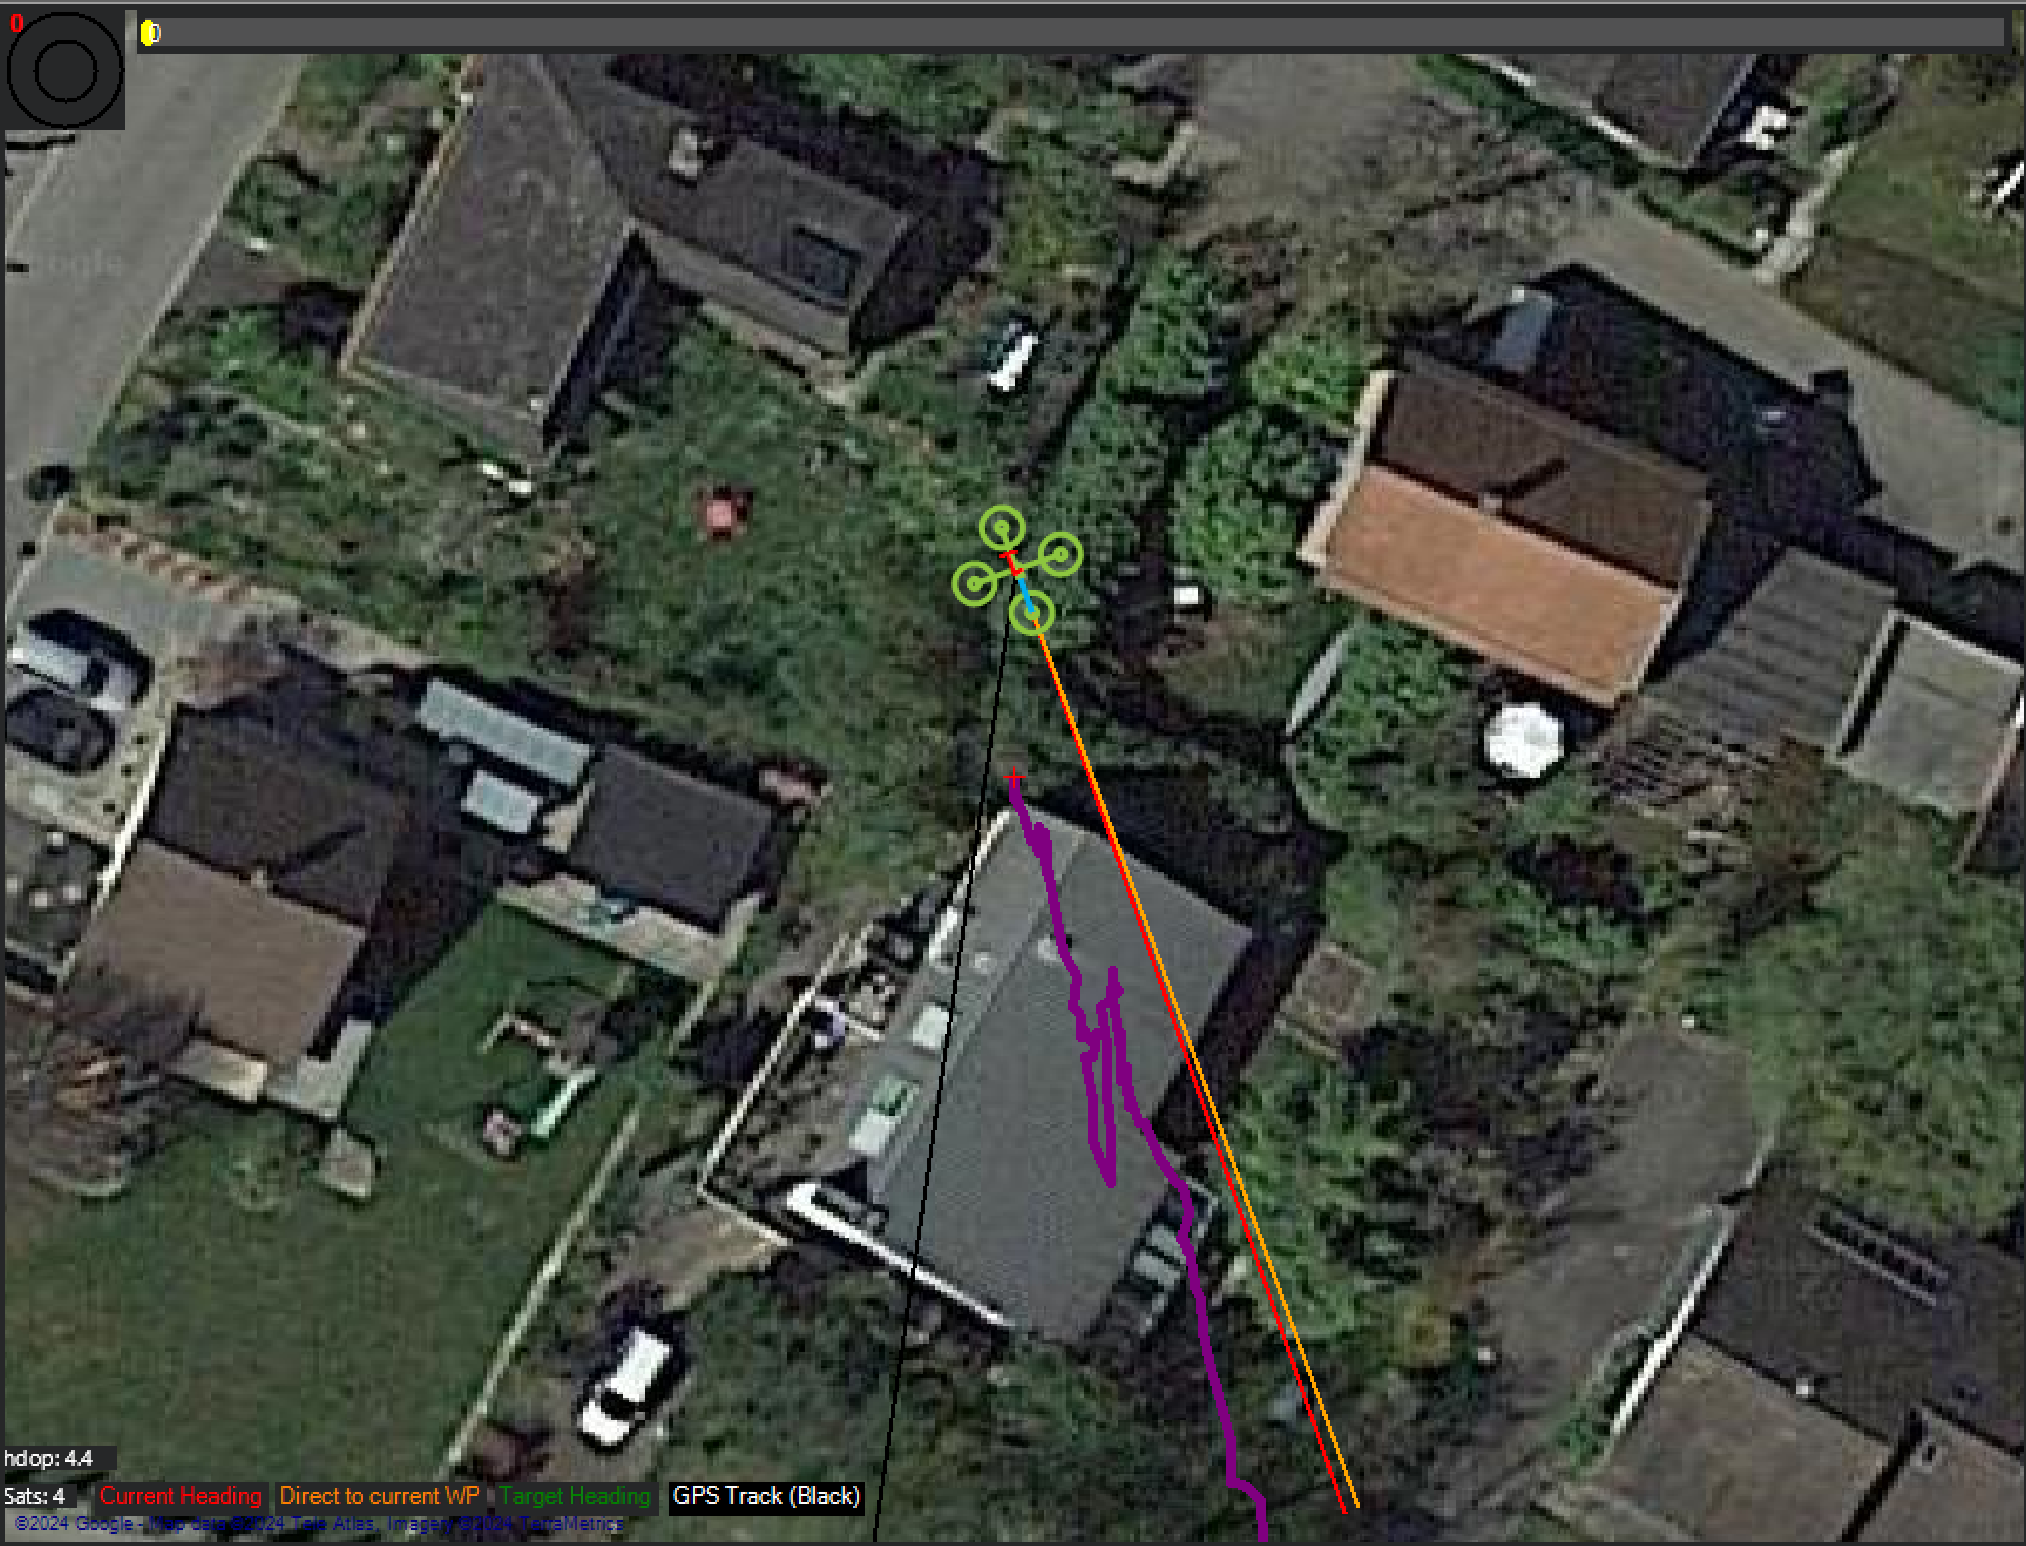
\includegraphics[width=\textwidth]{pictures/GPS_inside1}
		\caption{At home}
	\end{minipage}
	\hfill
	\begin{minipage}[b]{0.4\textwidth}
		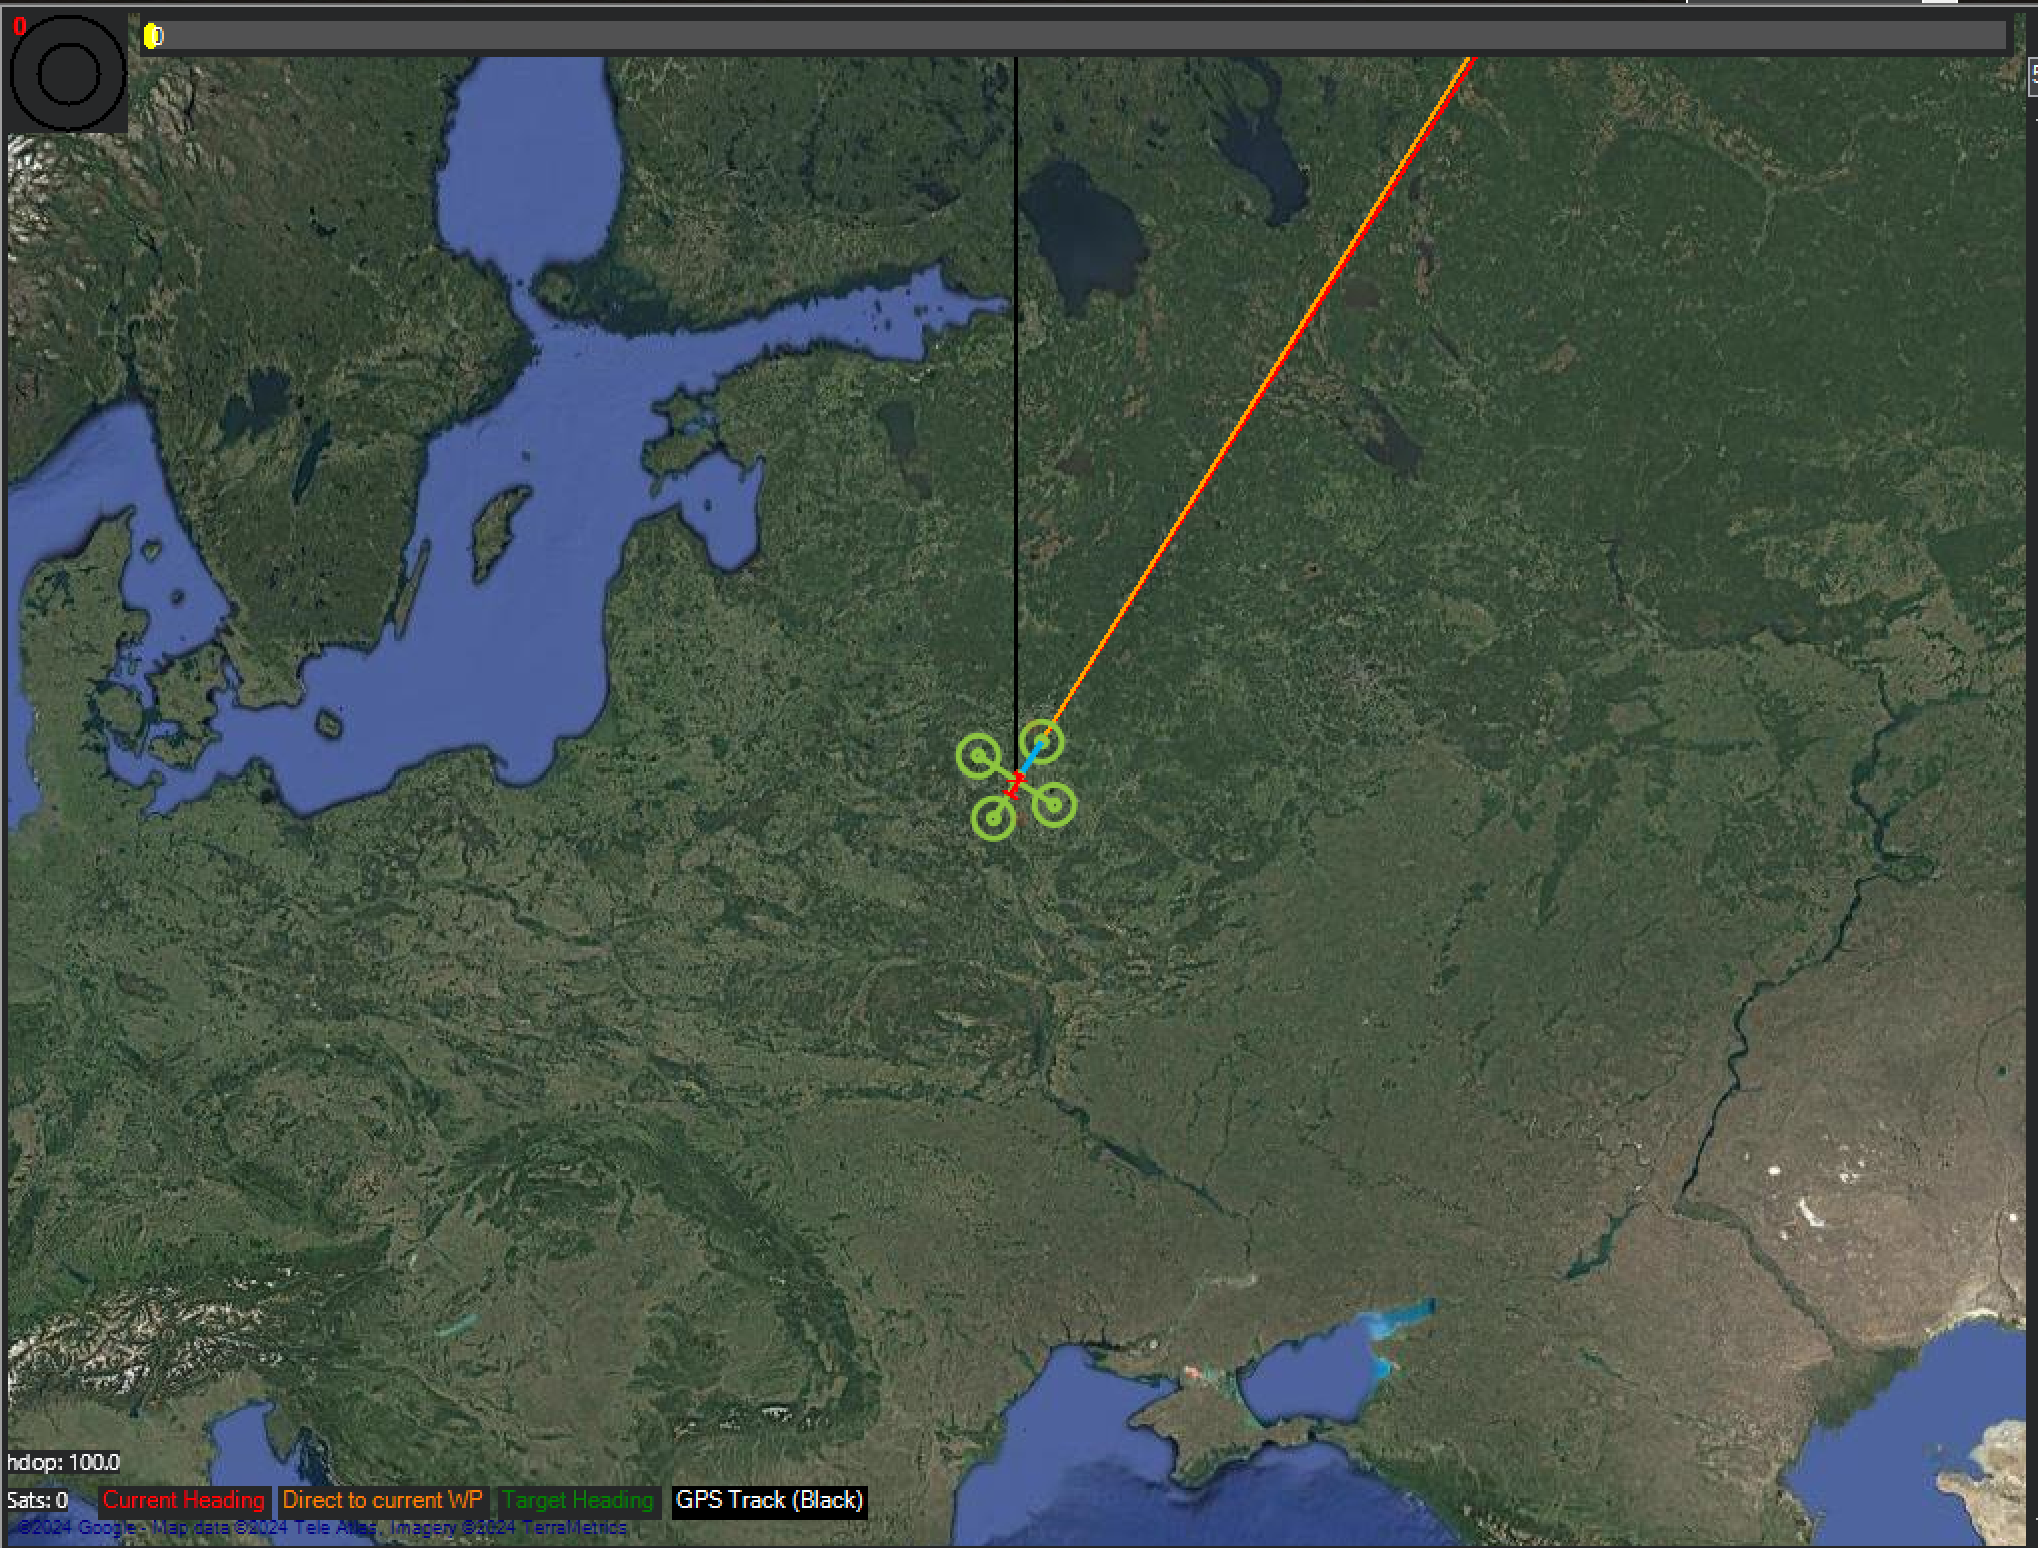
\includegraphics[width=\textwidth]{pictures/GPS_inside2}
		\caption{}
	\end{minipage}
\end{figure}

	 
	\subsubsection{Receiver/Transmitter}
	To get the connection between the receiver and radio I first followed the ExpressLRS\cite{expresslrsorg} page. I changed the \lstinline|Serial6_Protocol| to 23 and the \lstinline|RSSI_Type| to 3 for the receiver protocol. I also changed the \lstinline|RC_Options| to the correct bitmask.

\begin{figure}[h]
	\centering
	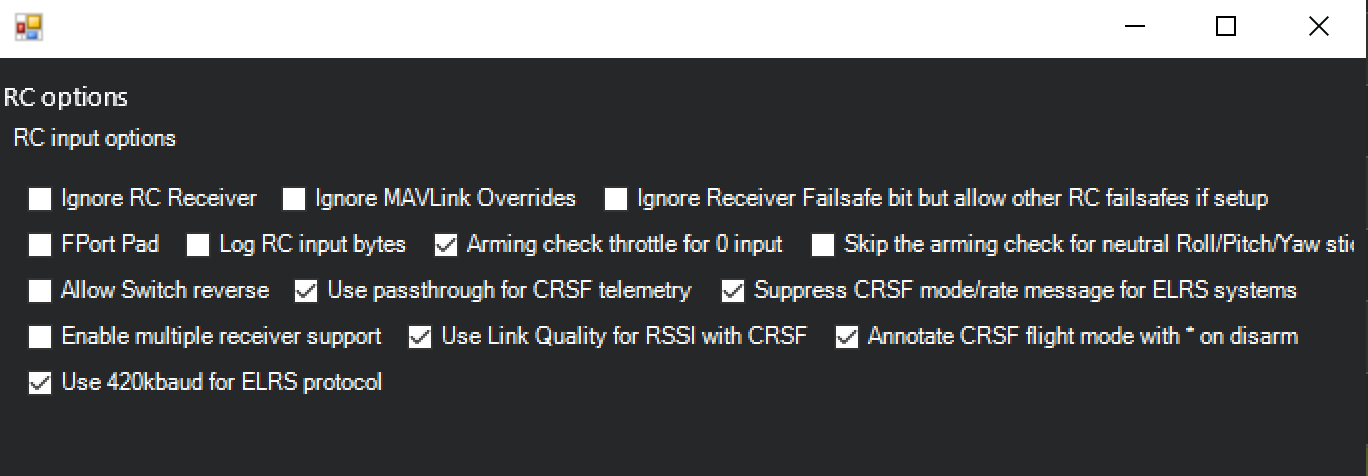
\includegraphics[width=0.7\linewidth]{pictures/bitmask}
	\caption{}
	\label{fig:bitmask}
\end{figure}

	The connection between the radio and receiver then worked, because the receiver had a constant blue light and the receiver said telemetry recovered after it was lost for a moment. However as it comes it did not have a connection to the Fc. I thought about changing the receiver from Uart6 to Uart 1, because Uart1 is the usual Uart for a receiver on the Kakute H7, but it would require a JST and more soldering. So I searched for a different solution. I looked at the Kakute H7 tab in the documentation and saw that for the Kakute H7 I needed to set \lstinline|Brd_Alt_Config| to 1 for the CRSF interface of the receiver. \lstinline|Brd_Alt_Config| is a Fc specific parameter so it makes sense that it did not come up in the search for a solution. 

	\subsubsection*{Battery}
	When I plugged in the battery the smoke stopper in between did not light up. The battery was not immediately recognized in MP and I needed to change the battery settings for the Tekko32 F4 4in1 I only needed to change the \lstinline|Batt_Monitor| to 4 the other parameters were already correct. I was now able to see the voltage and amperage of the battery.
	
\begin{figure}[h]
	\centering
	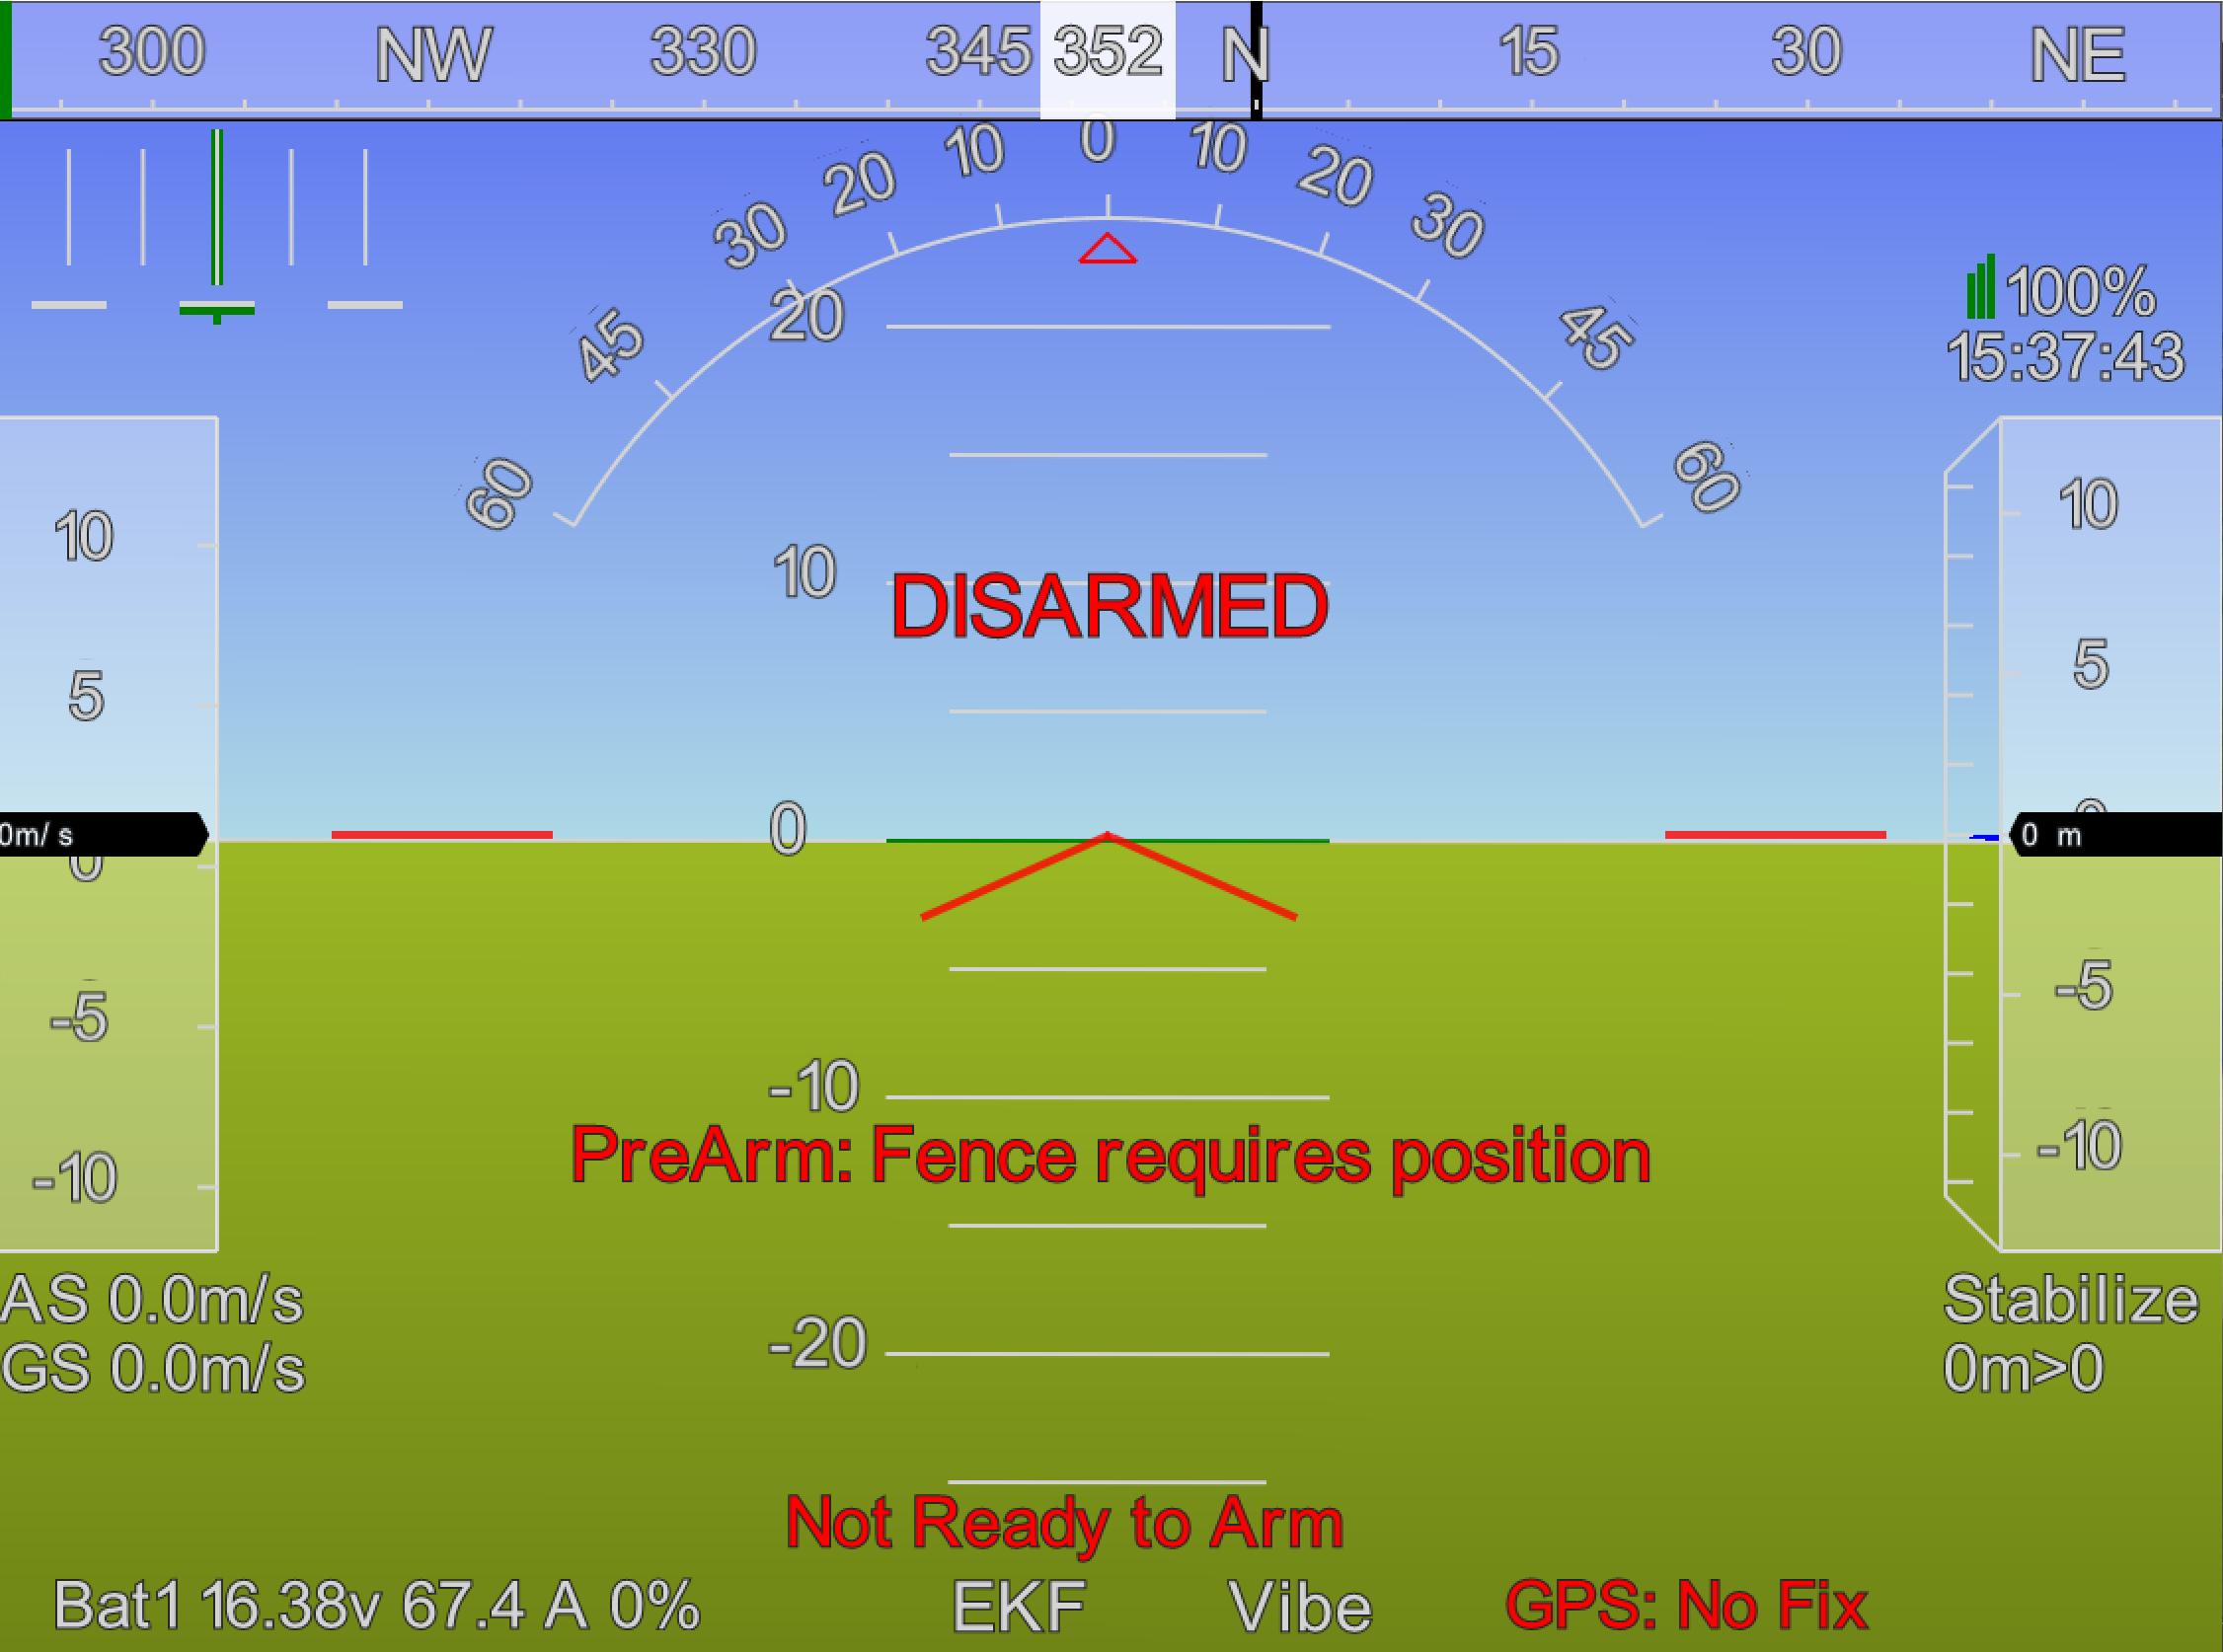
\includegraphics[width=0.7\linewidth]{pictures/Battery}
	\caption{}
	\label{fig:battery}
\end{figure}
	
	The only prearm check missing now is the compass calibration.(Figure 9\footnote{I'm currently inside and the GPS has no connection, but it works as soon as I'm under free Sky.})

\begin{figure}[h]
	\centering
	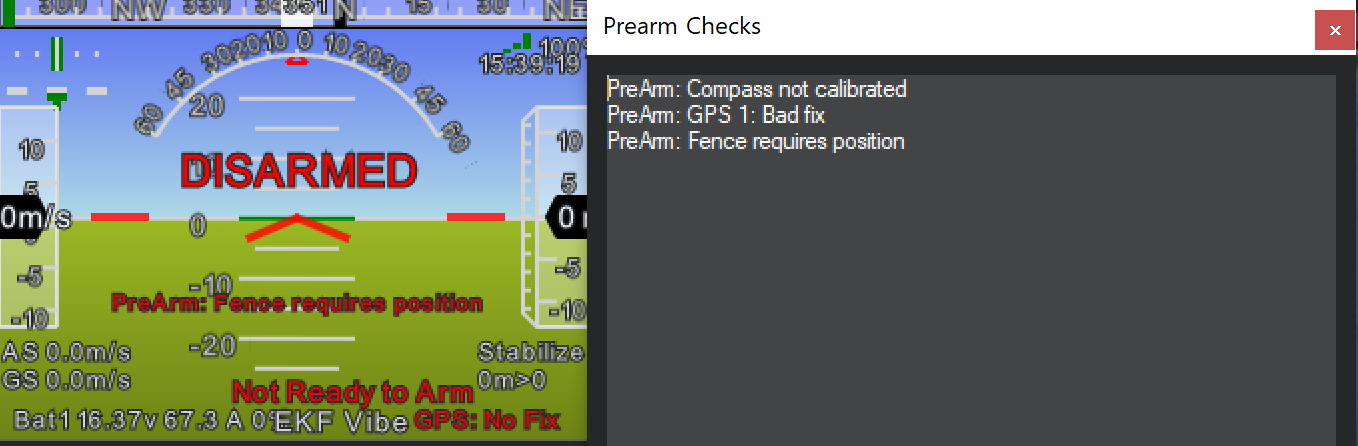
\includegraphics[width=0.7\linewidth]{pictures/prearmcheck}
	\caption{}
	\label{fig:prearmcheck}
\end{figure}


	\subsubsection{Motor Test}
	The motor test works correct after assigning the right position to the motors, because I'm using the M5-M8 ports instead of the M1-M4. I also needed to set \lstinline|Mot_PWM_Type| to dshot 600 for the 
	\\ Motor testing works after connecting assigning the right position to the motors and setting the mot\_pwm\_type to dshot 600. Dshot is just the digital protocol for communication between the Fc and ESC. After some time the motors began to beep, but after testing them again they stopped so it was most likely a inactivity warning. A new error also appeared called battery failsafe. This was caused by a unstable connection between the ESC and Fc and so the Fc took the connection from the computer as power source and had to little power to use the motors. 
	
	\subsubsection{Compass Calibration}
	I first tried to callibrate the compass inside, but it turns out that you need a good GPS lock. I went outside and tried calibrating the compass and it failed multiple times. I set the fitness to relaxed and it still failed. The Holybro docs\cite{holybrodocs} recommended to set the parameter \lstinline|Compass_Orient| to 6 for proper orientation. It failed again. I was definitely far enough away from metal or my computer which could influence the calibration.
	\\ I then fixed it temporarily by doing the large vehical MagCal, however this only took away the prearm message and did not really work. What I did not know at the time is that the ArduPilot documentation warns from using this calibration, because it can look as if it is correctly configured, but in reality the orientation is incorrect. 
	I later on needed to disassamble the copter anyway, because a wire between the motor and ESC came off and needed to be soldered on again, and put the GPS module directly onto the Fc and it worked using the normal compass calibration. 
	


	\subsubsection{Road to First Flight}
	All prearm checks are gone except the occasional magfield variance error(it disapeared completely after being able to calibrate the compass normally), which went away after positioning the drone further away from the computer. To arm
	% TODO explanation box of arm
	the drone I still needed to assign a switch on the radio. I did that by setting \lstinline|RC5_Option| to 153 which means to arm the drone when I flick the switch number 5. Even though there was no prearm check that failed I was not able to arm the drone, also when I disabled the parameter \lstinline|Arming_Check| it did not work. The Fc still rejected the force arm command from MP. The command however does not disable the geofence which I enabled some when earlier. I disabled it and was able to test the motors spinning on my bench. When I tried it with blades one of them hit one of the antennas from the receiver and tear it off. I was able to just attach it, but I'm not one hundred percent sure that this antenna is working. After this little hiccup a new prearm error appeared, crashdump bin detected. It comes from crashes with your drone to analyze what went wrong. 
	However, because I've only tested it on the bench, I concluded that it is insignificant and that I can delete it. But it is not just easily deleted and so I ignored it and did all the other prearm checks and then disabled \lstinline|Arming_Check|. I then armed the quadcopter and throttled up. The only thing it did was spinning on the ground, because some of the motors are turning in the wrong direction. Through a blog post\cite{blogcrashdump} I was also able to delete the crashdump.bin file by flashing new firmware onto the Fc. I tried to reverse the motors by using the reverse button in MP. It worked then by setting \lstinline|Servo_BLh_Auto| to 1 and open it in BLHeliSuite32\cite{BLHeliSuite32}. By using the reversed mode in BLHeliSuite32 I was able to get the right motors spinning clockwise. 
	
\begin{figure}[h]
	\centering
	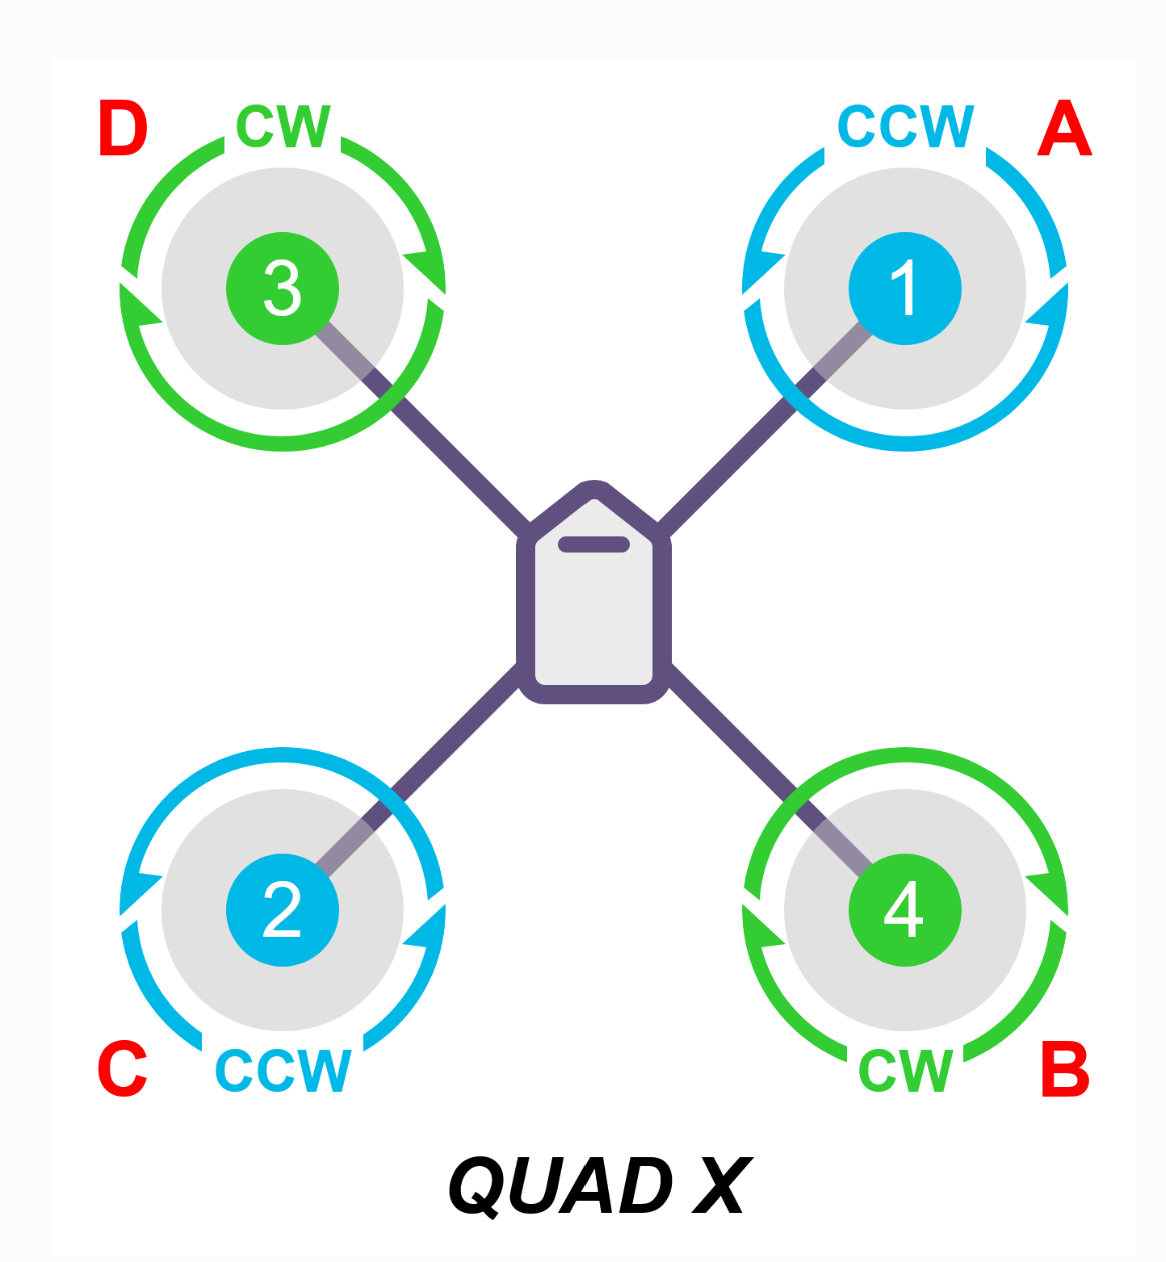
\includegraphics[scale=0.4]{pictures/quadx}
	\caption{Correct turning directions for my drone}
	\label{fig:quadx}
\end{figure}

	After arming the quad and pushing the throttle I was able to get the drone to fly, but it was shaking violently also known as wobbling and then somewhat crashed it into the ground causing the props to get minimal damage. I tried to tighten everything on the drone, because until that point everything was just somewhat loosely taped onto it, the wobbling still continued. Trying new and also the other props, as there could be a prop imbalance that causes the drone to wobble, had no effect. Through a video\cite{dronewobblevideo} about drone wobbling I came to the conclusion that my PID values are for a 9 inch drone not a 5 inch drone. 
	%TODO explanation box for PID
	After adjusting them via the intial tuning parameter quick adjustment settings the drone flew. But when I put the stick left the drone flew right and vice versa. I was able to put the \lstinline|RC2_Reversed| to 1, which reversed the controls. 
	

	\section{Results}
	\section{Discussion and Outlook}
	\section{Conclusion}
	
	\section{References}
	\printbibliography[
	heading=bibintoc,
	title={Bibliography}
	]	
	\section{Table of Figures}
	\comment{(short table on which every figure description with the page number is listed)}
\end{document}
